%&latex
\documentclass[a4paper]{report}
\usepackage{commons/commons}
\usepackage{commons/note_style}
\usepackage{commons/code_style}
\usepackage[normalem]{ulem}
\usepackage{comment}
\usepackage{titlesec}
\titleformat{\chapter}[display]
  {\normalfont\sffamily\big\bfseries\color{black}}
  {\chaptertitlename\ \thechapter}{5pt}{\huge}
%\excludecomment{figure}
\usepackage{amsbsy}
\usepackage{amstext}

\graphicspath{{./fig/}}
\begin{document}

%+Title
\title{Advanced Algorithm Quicksheet}
\author{Daniel D. Zhang, \\ Based on \textit{Algorithm Design by Kleinberg \& Tardos}}
\date{Winter 2015. \today}
\maketitle
%-Title

%+Abstract
%\begin{abstract}
%This is the notes for CSE 232A.
%\end{abstract}
%-Abstract

%+Contents
\tableofcontents
%-Contents
\chapter*{Preface}
Quicksheet. It only contains the most essential information. 
\section*{Acronyms}

\begin{obeylines}
\rih{Attr}. Attributes
\rih{Ptr}. Pointer
\rih{Mgt}. Management
\rih{idx}. Access key to array, that is array index; but it is not the database index.
\rih{est}. Estimate.
\rih{$\bot$}. Independent

\end{obeylines}
\chapter{Introduction}
Algorithmic problem solving.

{\obeylines
Technique. 
Examples. 
Writing.-  Plain English.
}

\section{Iterative Improvement}
Techniques.

Example: Stable Matching Marriage. People with free-will. 

Definition of \textbf{stability}:
Dataset: $w_1, w_2, m_1, m_2$.
\begin{align*}
w_1: m_1 > m_2\\
w_2: m_2 > m_1\\
m_1: w_2 > w_1\\
m_2: w_2 > w_1\\
\end{align*}
Stable matching pair: $m_i$ same preference, thus, $w_i$ gets the choices. 
\chapter{Divide \& Conquer}
\section*{Discussion}

Algorithm, starts from high-level, iterative refinements. 

MergeSort example: 

Divide procedure: 
Split the array $X$. Rough information: middle. Precise notation: $\lfloor\frac{n}{2}\rfloor$.

Merge procedure: 

Result invariant - non-decreasing. Taking the smaller element from the two sorted lists.

Corner case and base cases are important. 

\begin{align*}
T(1) &= 1\\
T(n) &= T(\lfloor \frac{n}{2}\rfloor) + T(\lceil \frac{n}{2}\rceil) +n \\
T(n) &= 2T(n/2)+n\\
T(n) &= 2(2T(n/4)+n/2)+n \\
\end{align*}

Let $n$ be a power of 2. 

Recursion tree method. Tree levels, tree nodes. 

Level $k$, $k=\lg n$. 

Reasoning process: 

Level - \# nodes per level - size per node - cost per node - cost per level

Precise answer:
$$
n (\lg n + 1)
$$

Variant: 
\begin{align*}
T(n) &= 2T(n/2)+2n \\
T(n) &= 3T(n/3)+n
\end{align*}
\begin{tabular}{lllll}
\hline\noalign{\smallskip}
\textbf{level} & \textbf{\#nodes per level} & \textbf{size per node} & \textbf{cost per node} & \textbf{cost per level}\\
\noalign{\smallskip}\hline\noalign{\smallskip}
0 & 1 & n& n &n \\
k & 3^k & n/3^k & n/3^k &n\\
\log_3 n & ...\\
\noalign{\smallskip}\hline\noalign{\smallskip}
\caption{Recursion tree}
\end{tabular}

Variant:
$$
T(n) = 3T(n/2)+n
$$
\begin{align*}
\sum_{k=0}^{\lg n} 3^k \frac{n}{2^k} \\
& = n \cdot 1.5^{\log_2 n} \\
&= n^{1+\log_2{1.5}} \\
&= n^{log_2 {3}}
\end{align*}


For increasing geometric sequence, keep the \textbf{last} term; for the decreasing
one, keep the \textbf{first} term.

\begin{align*}
T(n) = 4T(n/2)+n^2 
\end{align*}
\begin{tabular}{lllll}
\hline\noalign{\smallskip}
\textbf{level} & \textbf{\#nodes per level} & \textbf{size per node} & \textbf{cost
per node} & \textbf{cost per level}\\
\noalign{\smallskip}\hline\noalign{\smallskip}
0 & 1 & n& n &n \\
k & 4^k & n/2^k & (n/2^k)^2 &n^2\\
\log_3 n & ...\\
\noalign{\smallskip}\hline\noalign{\smallskip}
\caption{Recursion tree}
\end{tabular}

END OF DISCUSSION  

Algorithm and analysis of stable matching 
\
\section*{Discussion}
\subsection*{Truthfulness}
Stable Matching: lie to improvement self utility.

Follow the books the convention that men propose. Lying, it is possible to degenerate own outcome. Does lying always improve the utility? 

GS algorithm 1 dof: which free man to propose in \pyinline{while} loop. After proof, it always produces the SAME stable matching. Thus, it is possible to always improve by lying. 

\subsection*{Men-optimal}
Proposition: each man get the\textbf{ best stable} partner. Each woman get the \textbf{worst stable} partner. 

Proof by contradiction: $\exists m\in M$ does not get the best stable partner; thus he was rejected by the best stable partner. Chronologically, consider the first man rejection during the execution time. 

In matching $S$, $S$ is produced by GS:
\begin{align*}
& m-w'\\
& m'-w\\
& m: w >w'\\
& w: m' > m\\
&m': w > w''
\end{align*}

In $S'$: 
\begin{align*}
& m-w\\
& m'-w''
\end{align*}
, where $\exists w\in W, w=bestStable(m)$ is the best stable for $m$. 



Goal: $m'... w$ is a blocking pari in $S'$; thus $S'$ is not valid; thus to prove that $w\neq bestStable(m)$. 

Another level of proof by contradiction: 
Assume $m': w'' >w$. Then $m'$ proposes to $w''$ but rejected, which contradicts the $m$ is the \textbf{first} rejection. Thus, $m': w>w''$. Thus blocking pair in $S'$

\subsection*{Local Minimum}
$m*n$ matrix. $N=\max(m, n)$

\subsubsection*{Follow your nose} 
\textit{Follow your nose} algorithm: start with any cell \pyinline{cur}, if it is a local min, found; else, at least one \pyinline{cur < nbr}, then \pyinline{cur = nbr}. - Iterative improvement. 

Does it terminate? There is no infinite loop $\infty$, proof by contraction, some cell strictly $>$ itself.

When it terminates, it found because all conditions met. 

This algorithm proves the existence of the local minimum. But this algorithm is $O(mn)$.
\subsubsection*{Improvement}
Binary search in 1d, divide into 2 parts. Binary search in 2d - divide into 4 parts. 
Check the border of 4 parts (squares). 

The sub-problem must have exact pattern and only differs in size. And we want to have balanced parts rather than size-unbalanced parts. 

When if we found local min in a part on the border of the part, can we ensure this local min is actually the local min considering the boundary that is thrown away when entering into this part. Thus, what we need is a clean cut. 

\subsection*{Hidden surface}
Do the analogy. 
Compared to \textbf{merge sort}, this problem has no clear input and data structure (repr). Visible surface is abstraction without concrete data structure. What is the data structure used to repr the visible surface. What you are merging the visible surface. 

$L_1, ..., L_n$ repr as:
$$
y=m_ix+b_i
$$

To repr the visible surface: indexes of lines give the \textbf{sequence} to calculate the intersecting point $\in$ surface. 

In the merge sort, there are two increasing sequences. What are  the ``increasing'' surfaces? Then how to merge the two ``increasing'' surfaces?

END OF DISCUSSION

\section{Integer Multiplication}
\section{FFT}
From integer multiplication to polynomial multiplication 
\begin{align*}
& A(x) = \sum_{i=0}^{n-1} {a_i x^i}\\
& B(x) = \sum_{i=0}^{n-1} {b_i x^i}\\
& C(x) = A(x)*B(x) = \sum_{i=0}^{2n-2} {c_i x^i} \\
& \text{, where } c_i = \sum_{j=0}^i {a_j b_{i-j}}
\end{align*}
Notice that sum of indexes is the same.

Horner's method  can reduce the complexity of eval the value of the polynomial. 
\begin{align*}
4x^3+3x^2+2x+1 &=  \\
&((4x+3)x+2)x+1
\end{align*}

Fourier transformation: frequency domain $\leftrightarrow$ time domain. Coefficient domain $\leftrightarrow$ value domain. 

Eval $A(x), B(x), C(x)$ using $x_1, ..., x_n$. And you have the freedom of choosing $x_i$. You can evaluate the expressions when  $x_i=1$ and $x_i=-1$, you can easily eval; $\Ra$ we want $\forall i, x_i$ is 1 or -1. 

\section{Closet pair}
$(x_i, y_i), 1\leq i \leq n$. Find $i\neq j$ s.t. $(x_i-x_j)^2+(y_i-y_j)^2$ in min.

\subsection{1-D problem} 
Sort and compare neighboring points. 

\subsection{2-D with a narrow band}
Naive sort by $x$-coordinate, counter example: $(0, \delta), (\varepsilon,-\delta), (2\varepsilon,\delta)$

Slight deviation from the 1-D line. All points fall in a strip $2\delta$. 

But can the $\delta$ be far apart? Try to figure out the upper limit of $\delta$.

After getting $\delta$, divide the band into cells of length $\delta$. 
\begin{python}
----------
|_|_|_|_|_| delta
| | | | | | delta 
----------
\end{python}

We need to find the closet pair in this narrow band, We stuck here for finding close pair in band because we haven't define the \textit{algorithmic meaning} of $\delta$, 

\subsection{2-D D\&C} 
Target: total $O(n \lg n)$, merge $O(n)$. 

$\delta = \min(\delta_1, \delta_2)$, where $\delta_1$ is from the right sub-problem, and $\delta_2$ is from the left sub-problem. 

Does there exist a pair of point $l \in \mat{L}, r \in \mat{R}$, s.t. $d(l, r) <\delta$. 

Filter out the impossible (informational useless) points. 
\begin{enumerate}
\item \textbf{Outside the band}: $d(l, r)<\delta \Ra$ filter out points reside outside the separating line $L$ band of $\pm\delta$ (rather than $\pm0.5\delta$) along the $x$-axis. Form the band $\mat{S}$. 
\item \textbf{Inside the band}: $d(l, r)<\delta \Ra$ for each scanning point $cur$,  filter out points reside outside the $\pm\delta$ along the $y$-axis; only keeps neighbors. \textbf{Limited search space}. After filtering, find the upper bound of number of neighboring points.  
\end{enumerate}

If you divide the band into finer cells of length $\frac{\delta}{2}$. For each point $cur$, there are only $O(16-1)$ points that is possible to have $d(cur, nbr)<\delta$ within the 16 neighboring cells respectively. $+4: 4^2$. Then reduce the search space into $O(16-1)$ along the $y$-axis. Notice that $\forall cell$, at most 1 point $\in cell$ due to the $cell \in \mat{L}$ or $cell \in \mat{R}$.

Although unnecessary, we can further reduce the search space, if the $cur\in \mat{L}$, no need consider $\{nbr|nbr\in \mat{L}\}$, the only need to consider $4^2/2=8$ neighbors, up 4 and down 4. Thus need to compare 8 $nbr$ in $S_y$. 

\subsection{Write Proof}
How to write the proof:
\begin{enumerate}
\item High-level ideas
\begin{enumerate} 
\item \textbf{Notations}. Define the mathematical notations rigorously. 
\begin{enumerate}
\item Let $S_L' = \{p|p\in S_L, |p_{x}-x_{mid}|\leq \delta) \}$, where $p_x$ is the
$x$-coordinate of $p$.
\end{enumerate}
\item  \textbf{High-level}. The detailed can be suppressed since assume background knowledge. Thus, provide high-level details rather than implementation details
\begin{enumerate}
\item ``while keeping track of the $min$''.  
\item Let $S_L$ sorted by $x$-coordinate in
what order.
\end{enumerate}
\item \textbf{Sections}. e.g. D\&C - 1) base case 2) divide 3) merge 
\end{enumerate}
\item Proof
\begin{enumerate}
\item \textbf{Target}. What we found is what we want. - the target is only in the subsets; why we can
filter out other sets.
\item \textbf{Numbering} Numbering the arguments in the ideas, easier to ref.
\end{enumerate}
\item Time complexity
\begin{enumerate}
\item \textbf{Track}. Track and argue the time complexity. [$O(N)$]
\item \textbf{Recursion}. Solve the recursion equation 
\item \textbf{Const}. Constant matters
\item \textbf{Graph}. Verbal is necessary while graph is not sufficient, although graph assists the math notations. 
\end{enumerate}
\end{enumerate}

\subsection{Dimension}
for high dim:
$$
2^k n \log n 
$$
\section{Majority element}
find $x$ in array $A$ with length $n$ s.t. $cnt_x > n -cnt_x$. 

Find a pair $(a_i, a_j)$ in $A$, if $a_i \neq a_j$, delete both from $A$. it still holds that: $C^{A'}_x > |A'|-C^{A'}_x$. Proof, since $a_i\neq a_j$, at most 1 of them equals $x$, then $C^{A'}_x$ decrements at most by 1, $|A'|$ decrements by 2. 

To find such pair $(a_i, a_j), a_i\neq a_j$, linear time one-pass algorithm. That's why \textit{Moore's voting algorithm} is correct. 

Proof: At any time in the execution, let $A'$ be the prefix of $A$ that has been processed, if $counter>0$, then keep track the candidate $majority$'s counter, the $majority$ is the majority number of $A'$.  If $counter =0$, then for $A'$ we can pair the elements s.t. are all pairs has distinct element. Thus, it does not hold that $cnt_x>n-cnt_x$; thus $majority\in A'$.

What if there no majority number. Proof the relaxed problem (i.e. majority number must exists) as above; then handle stricter problem. 

\textbf{D\&C}. Need to keep track the number of matched pair; need to handle the odd-length subset $\Ra$ more complicated. 

Why simple find the majority in subset is not sufficient: 7 $x$, 6 $y$. 
\begin{align*}
[(x, x) (x, x) (y,x)][(y, x) (y, x) (y, y)][y]
\end{align*}

After conquer:
\begin{align*}
x | y|y
\end{align*}
\subsection{Skyline}
Similar to visible surface, but easier. 

\textbf{repr}. Define the repr. The number of building is $n$. The building is represented in $(s_{i}, e_{i},h_{i})$, s.t. in the interval $[s_i, e_i)$, the height is $h_i$. 

What is the repr for the skyline? A list = $[(s'_i, e'_i, h'_i)]$


Use D\&C. When the skyline changes? At start and end. 

\textbf{Preprocess}. Sort the building by $s$. 

\textbf{Divide}. Divide into $B_1, B_2$ and conquer them. 

\textbf{Merge}. Merge efficiently $B^1, B^2$, scan the $x$ from either $B^1, B^2$, $h_x$ at $x$ is $h_x=\max(h^1_x,h_x^2)$. Sorting building by $s$ can make it easier. Use $e^1_{end}$ and scan the points from $B^2$

\chapter{Greedy Algorithm}
Agenda:
\begin{enumerate}
\item Scheduling max number of intervals 
\item Minimizing max lateness
\item Cache replacement policy
\end{enumerate}
\section{Events scheduling}
\textbf{Definition} of the problem: Max number of intervals without overlapping. 

\textbf{Notations}
$$
[s_i, f_i), \text{ where }1 \leq i \leq n
$$

\textbf{Ideas}
\begin{enumerate}
\item select the interval with min degree of conflicts 
\item select the interval with shortest duration 
\item select the interval with min start time 
\item select the interval with min end time
\item select the interval with latest start time (dual with 4, same as 4 and just look a the input arrays in a reversed order)
\end{enumerate}

\textbf{Proof} idea 4. Proof by contradiction and proof by induction. Greedy solution $\mat{G}$, optimal solution $\mat{O}$. 
\begin{align*}
& \mat{G} = \{G_1, G_2, ..., G_k\}  \\
& \mat{O} = \{O_1, O_2, ..., O_l\} \\
& k > l 
\end{align*}

Sort $\mat{G}, \mat{O}$  by finish time. 

Technique ``\textit{Exchange Method}". rearrange the $\mat{O}$ to look like $\mat{G}$, and to the end $\mat{O}, \mat{G}$ are the same (i.e. $|\mat{O}|=|\mat{G}|$). 

For the 1st elt:
\begin{enumerate}
\item if $G_1=O_1$, then move to the next index
\item else, $G_1.f < O_1.f$ since greedy; and then exchange $O_1$ with $G_1$ without conflicting other $\mat{O}[2:]$. 

$\forall i>1, O_i.s > O_1.f >G_1.f$
\end{enumerate}

For the 2nd elt: Since after exchange, $G_1=O_1$, we truncate the first element, thus the problem $\mat{O}[2:], \mat{G}[2:]$ can be solved similar as  $\mat{O}[1:], \mat{G}[1:]$.

After iteratively applied, $\mat{G}[1:k+1]=\mat{O}[1:k+1]$.

After consuming all the $k$ element, the way of greedy works (select the earliest end time \textit{until} there are no more), you can argue that there is no more $O_{k+1},..., O_l$. If there are more, the greedy algorithm will continue the selection which contradicts that the greedy has stopped.

\section{Exercise}
General methods to proof greedy algorithm
\begin{enumerate}
\item Exchange method
\item Stay head 
\item Optimal substructure 
\end{enumerate}
\subsection{Changing road conditions}
\begin{align*}
& G_i \ra G_{i+1}\\
& P_i \\
& G_i, P_i, \sum_{i=0}^b l(P_i)+k \cdot change(P_0, ..., P_b)
\end{align*}
, where $k$ for the penalty of changing the path. 

The $t$ changes, but the previous path does not change, but it may not be the shortest path. 

Cannot to D\&C since the two subproblems (divide the Graph into two halves) influences each other. There is no clear boundary btw two subs. 

\textbf{Relexation}. Take a simpler version of the problem, regardless the previous sequence, for the subsequent subs, you get the min cost. 

\subsection{Timing circuits}
Data structure. Goes up \& down. repr
\begin{enumerate}
\item Pointers
\item Heap (heapq)
\end{enumerate}

BFS, and set the length. 

Don't need to write pseudo-code. 

Ideas:
\begin{enumerate}
\item start at leaf level. 
\item start at root level.
\end{enumerate}

Produces $\forall$ root-to-leaf path lengths are equal (intermediate nodes doesn't matter) and with min sum of edge lengths. 

Observations: 
\begin{enumerate}
\item The greedy algorithm produces the with zero-skew result s.t. the root-to-leaf path length equal to the maximum root-to-lead path length; and minimal length. The extra property is - max original root-leaf path. 
\item defining this additional property that can do \textit{recursion}.
\end{enumerate}

Procedure: 

1 level down, make two trees rooted at left child and right child be min-zero-skew-max-length trees; and adjust root to left and right child length to the the max-length from root-leaf path. 


Proof the correctness of idea: 
TODO

\subsection{Time-varying MST}
Kruskal's algorithm is sufficient. less complex than Prim's.

Exploit Kruskal's algorithm property that. 

Find the changing points (calculus). between the changing points, the relative order of the $E$ does not change. 

Once the order changes, re-run the Kruskal. (no need to optimize). Just need polynomial algorithm. 

The problem is reduced to find the changing points. 

\section{Optimal substructure}
Proof technique for greedy algorithm and dp.

a problem is said to have optimal substructure if an optimal solution can be \textbf{constructed} efficiently from \textbf{optimal} solutions of its \textbf{subproblems}. This property is used to determine the usefulness of dynamic programming and greedy algorithms for a problem.

e.g. maxima number of intervals. 

Find optimal solutions in subproblem, and combine the the solution. 

\section{Minimize Max Lateness}
Tasks $(t_i, d_i)$, duration and deadline. 

Schedule $(s_i, f_i)$, where $f_i=s_i+t_i$, start time and end time. All jobs can be scheduled. The goal is to minimize the max lateness: 
$$
\min L = \min(\max_i l_i), \text{ where } l_i=\max(0, f_i-d_i)
$$

Analysis: no reason for gaps between tasks.

\textbf{Ideas}:
\begin{enumerate}
\item Min $d_i$ first
\item Min $t_i$ first, counter example: $(2, +\infty)$, $(2, 2)$
\item Max $l_i$ first 
\end{enumerate}

\textbf{Strategy}:

The correct answer is Min $d_i$ first. 

Prof by contradictions + \textit{Exchange Method}

Consider the greedy solution $\mat{G}$ s.t. scheduled as $d_1 \leq d_2\leq ...$. Consider a opt solution $\mat{O}, \exists i,j, d_i > d_j$ s.t. $i$ is scheduled earlier. 

Exchange method: exchange $i, j$, but hard to analyze for the schedules $\mat{O}[i+1:j]$. However, If $i, j$ is adjacent:
\begin{figure}[!htp]
\centering
\subfloat{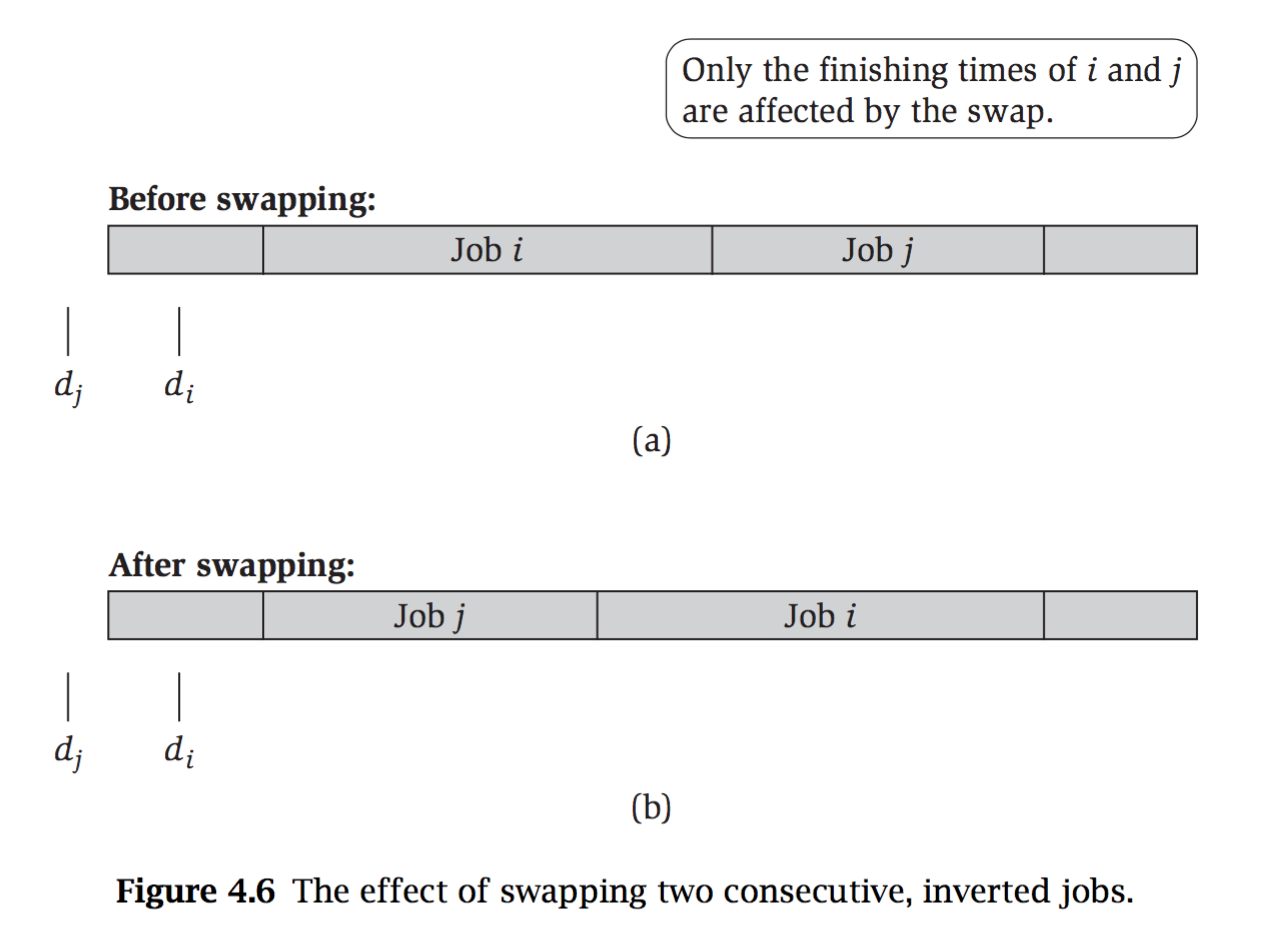
\includegraphics[scale=1.0]{4_6}}
\caption{Consecutive intervals}
\label{fig:4_6}
\end{figure}

Job j is earlier, lateness can only be reduced. Only need to prove $l_j>l'_i$.
\begin{align*}
& \mat{O} \text{ is worse than } \mat{O'} \\
\Leftarrow & \max(l_j, l_i) > \max(l'_j, l'_i) \\
\Leftarrow & \because l_j > l'_j, \therefore \text{only need to prove } l_j>l_i'\\
\Leftarrow &
\end{align*}
Lateness of job j in \mat{O} $l_j= f_j - d_j$

Lateness of job j in \mat{O'} $l'_j= f'_j - d_j$

$l'_i=f'_i - d_i=f_j-d_i$. Thus, $l'_i<l_j$



\begin{align*}
&\because l_j > l'_j, l_j>l'_i\\
\end{align*}

Then like bubble sort.

\chapter{Dynamic Programming (DP)}
\section{Min cost of pair-wise sum}
Operation: Sum pair-wise 

Sum all. Goal: get the minimize cost $c\triangleq A_i+A_j$.

Analysis:

Take 2 min elements, and sum them up, del the 2, put back the sum. Repeat this process. Thus, use heap. 

Proof. TODO

\section{}
Given intervals $A$: $[s_i, f_i), w_i\geq 0$, where $w$ is the weight. 

\textbf{State definition}:
$M(i)=$ max sum of weights of a non-overlapping set of jobs where the jobs come from $A[i...n]$

Least relaxed problem: $M(1)$. Most related problem $M(n)$.

\textbf{State transition functions}:
\begin{align*}
M(i) = \min&\Big( w_i+M(j) \text{, where $j$ is the earliest index s.t. } s_j\geq f_i\\
&M(i+1)\Big)
\end{align*}

Notice that, $M(i)$ is monotonous.

\section{Top-down dp}
solve the problem in brute force, find same subs, cache them, reduce exponential to polynomial. 
\end{document}
